
\chapter*{Introduzione}

Da qualche anno a questa parte sono stati sviluppati e messi in commercio dispositivi per la realtà virtuale, alcuni dei quali sono la Nintendo \textbf{Wii}, il \textbf{Kinect} della Microsoft o l'\textbf{Oculus Rift} sviluppato da Oculus VR. Periferiche come queste sono dette \textbf{NUI}, “Natural User Interface”\cite{NUI}: essenzialmente sono interfacce che hanno lo scopo di rendere più realistica l'interazione con sistemi virtuali, permettendo all'utente di immergersi nell'ambiente virtuale. Il termine naturale è dovuto al fatto che l'interfaccia può essere utilizzata senza l'ausilio di un dispositivo fisico, ad esempio compiendo movimenti e gesti naturali, in modo da rendere trasparente il suo funzionamento all'utente.

La Wii permette, tramite il suo telecomando, di utilizzare indirettamente il corpo umano come dispositivo di input di comandi. Il Kinect utilizza dei sensori a infrarossi e una telecamera per rilevare il corpo umano e registrare direttamente i suoi movimenti, trasformandoli in comandi di input. L'Oculus Rift è un visore che contiene due schermi per la visione tridimensionale; inoltre presenta dei sensori che riconoscono l'orientamento della testa, i cui movimenti sono tradotti in rotazioni della telecamera virtuale all'interno dell'applicazione, in modo da rendere più immersiva la visione.

Il progetto trattato in questa tesi mira ad emulare dispositivi di questo genere, utilizzando semplicemente un computer e una webcam. La posizione del volto, rilevata elaborando le immagini acquisite tramite la webcam, determina la prospettiva con cui viene visualizzata una scena tridimensionale, con lo scopo di collegare la telecamera virtuale agli occhi dell'utente. L'obiettivo finale è quello di generare l'illusione della presenza di profondità all'interno dello schermo e di creare, in condizioni ottimali, un effetto tridimensionale senza l'utilizzo di occhiali appositi.

Dato l'utilizzo di dispositivi di qualità medio-bassa, l'effetto generato non è paragonabile a quello che può essere prodotto da sistemi più efficienti e dedicati allo scopo, tuttavia sono stati raggiunti comunque risultati notevoli.

Il progetto è stato sviluppato impiegando i seguenti software e librerie:
\begin{itemize}
\item \textbf{OpenCV}, per il rilevamento del volto.
\item \textbf{OpenGL}, per lo studio di fattibilità e per lo sviluppo di un prototipo.
\item \textbf{Blender}, per la creazione di scene 3D.
\item \textbf{Ogre3D}, per un miglioramento dell'applicazione in termini di grafica ed efficienza.
\end{itemize}

Nei primi due capitoli di questa tesi sarà fatta un'introduzione sulla realtà virtuale e si parlerà delle tecnologie utilizzate, spiegando le basi delle trasformazioni usate nella maggior parte delle applicazioni grafiche per renderizzare a schermo scene tridimensionali. Negli ultimi due capitoli sarà trattato il progetto sviluppato e saranno mostrate le problematiche riscontrate, con le possibili soluzioni.



\begin{figure}[htbp]
\centering
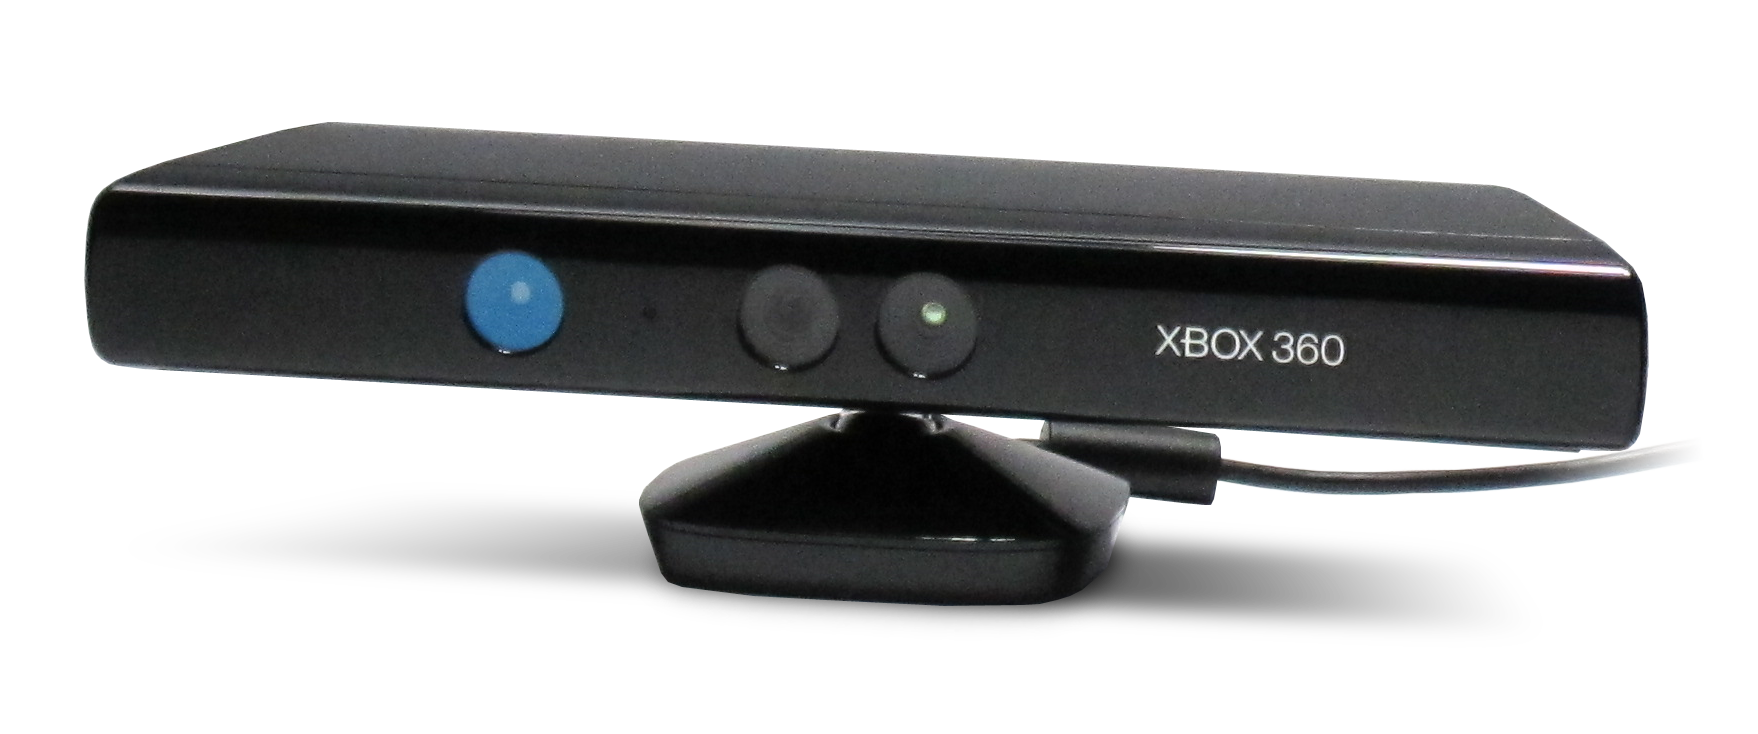
\includegraphics[width=0.4\textwidth]{images/introduzione/kinect.png}
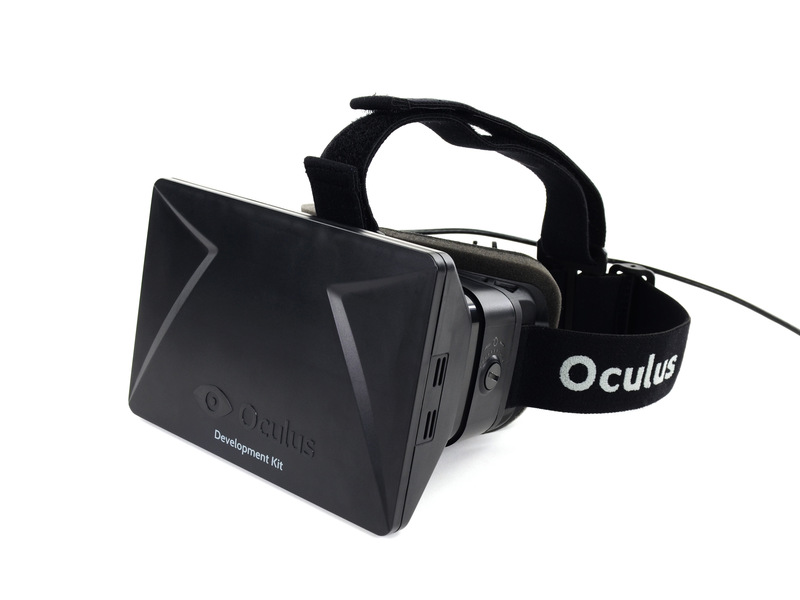
\includegraphics[width=0.4\textwidth]{images/introduzione/oculus-rift.jpg}
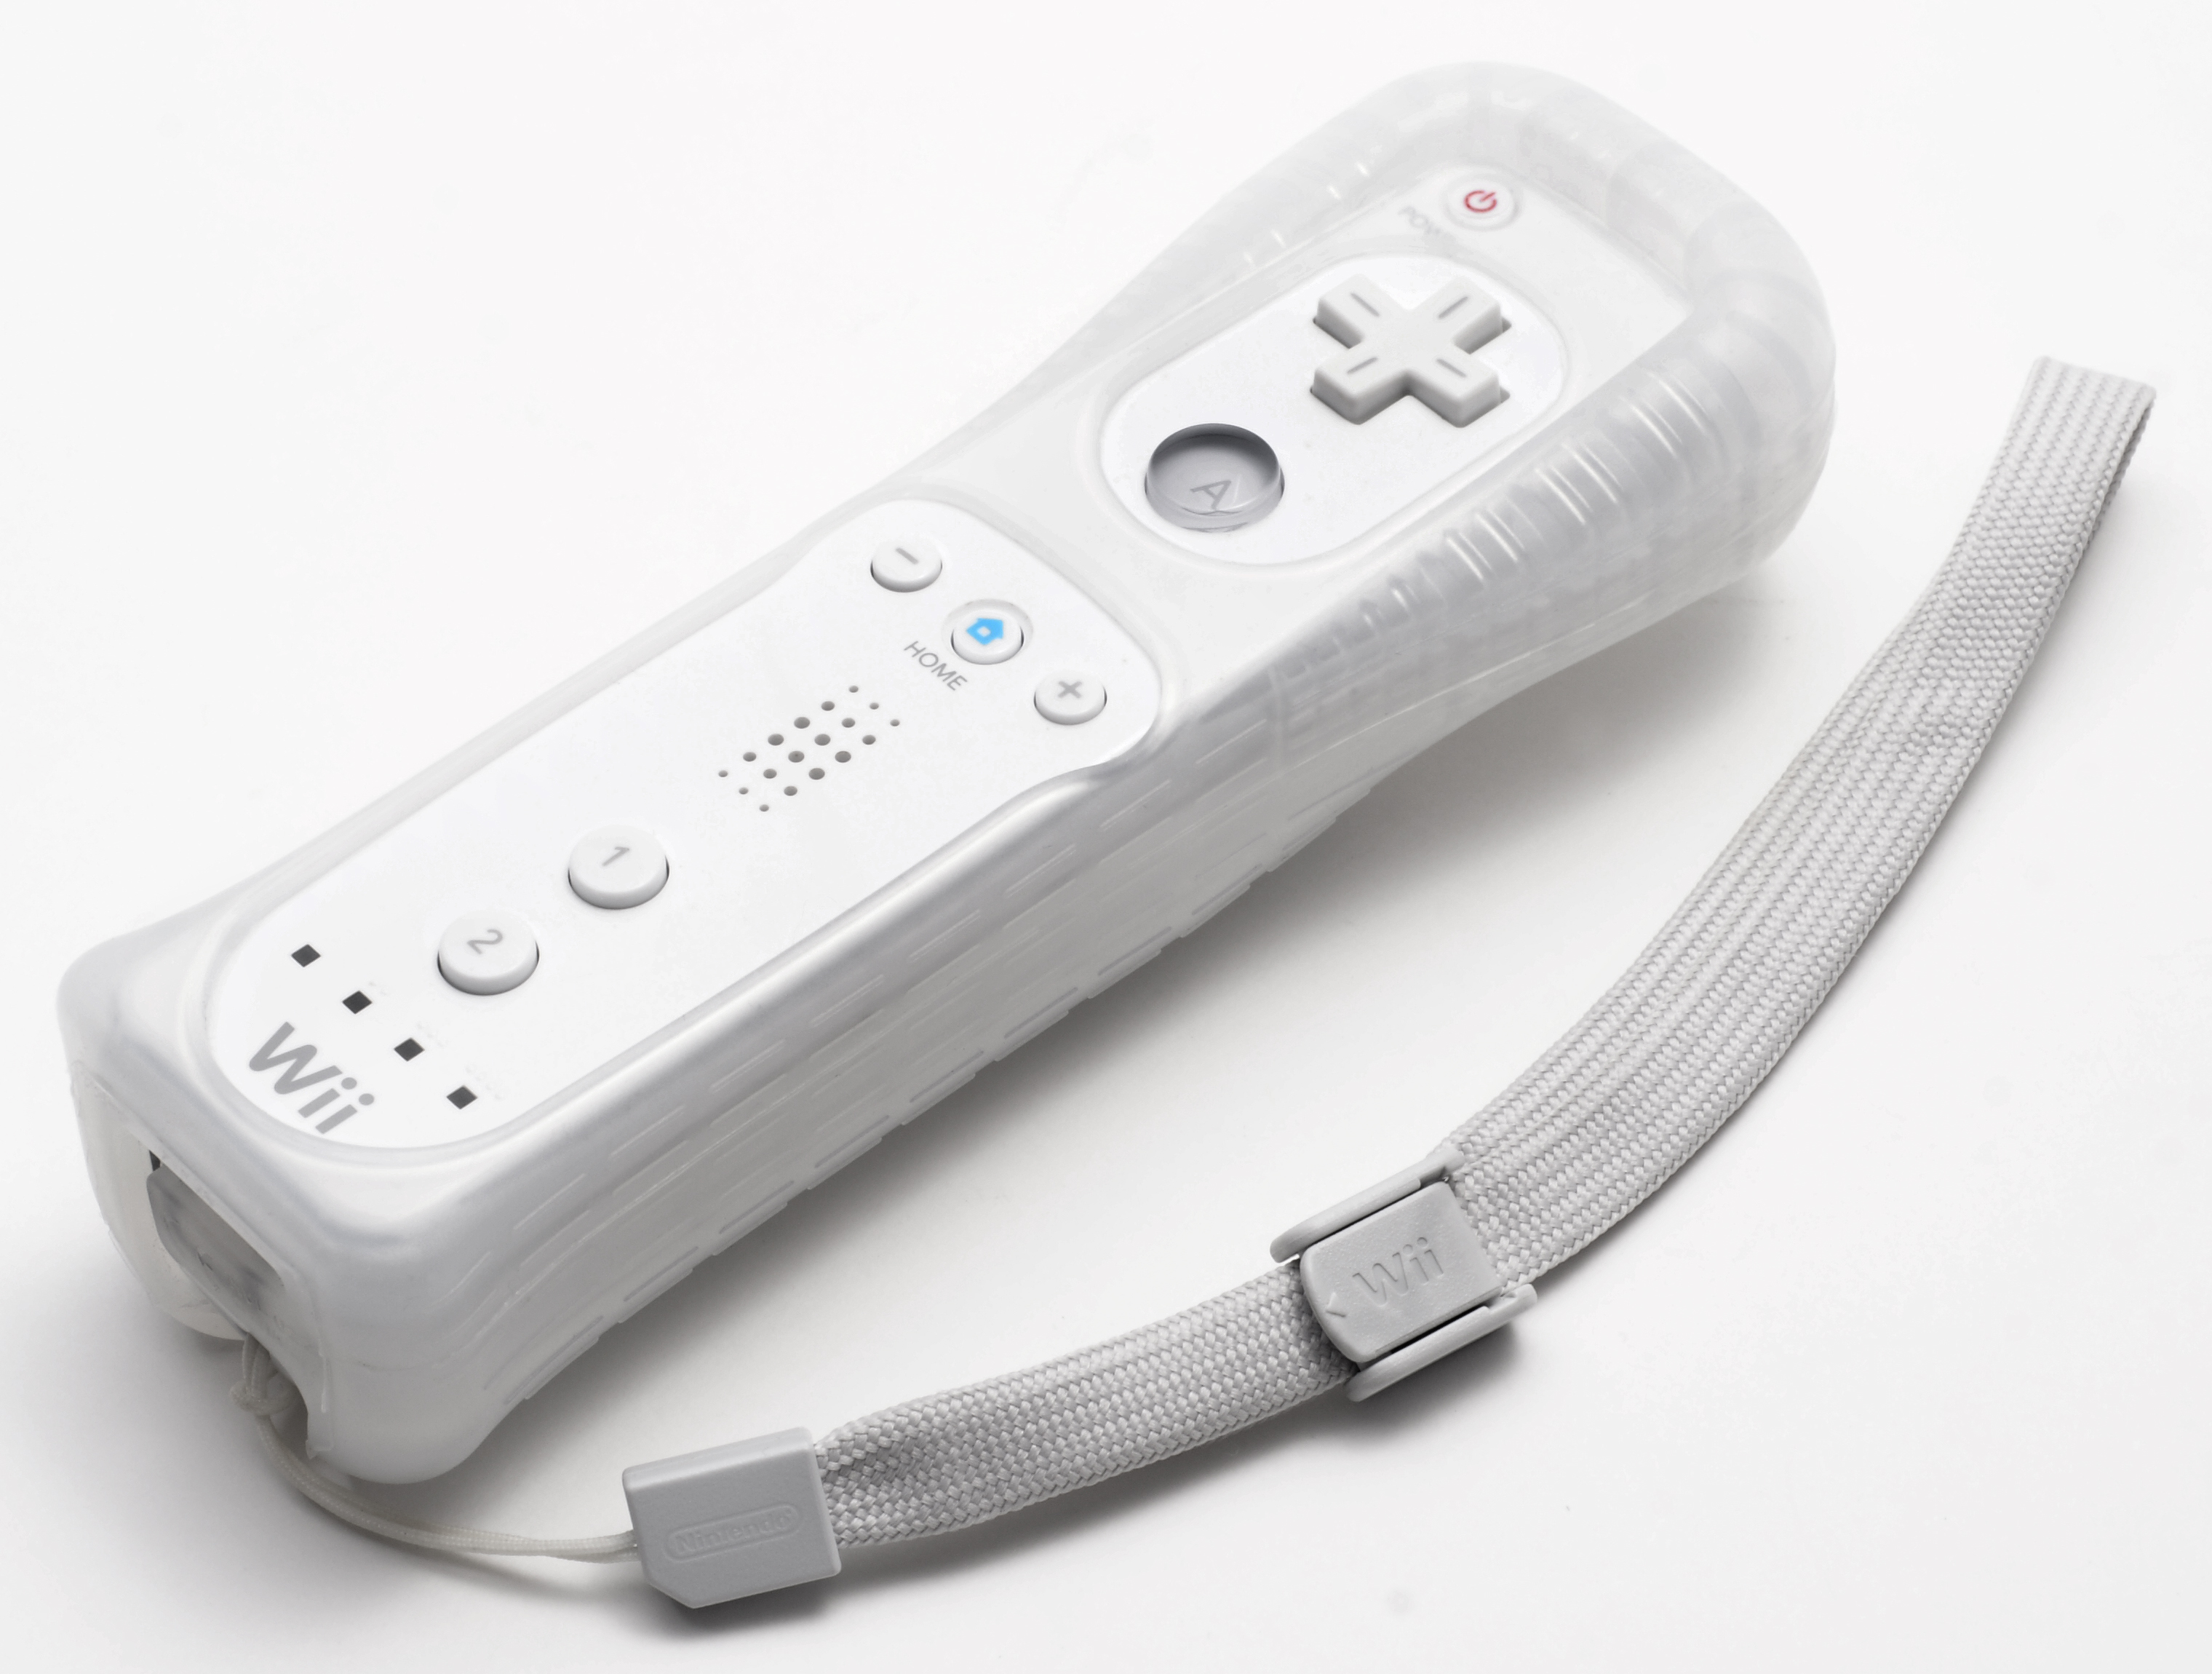
\includegraphics[width=0.4\textwidth]{images/introduzione/wii.jpg}
\caption{Esempi di NUI}
\end{figure}
